\chapter{Линейные модели}
\label{chap:linear_models}

\begin{supportbox}{Об этой главе}
Программирование программного обеспечения осуществляется путем выбора соответствующей последовательности примитивных операций для решения задачи. По аналогии, построение модели осуществляется путем выбора правильной последовательности \textit{дифференцируемых} блоков. В этой главе мы представляем самый простой возможный блок, так называемые линейные модели, которые предполагают, что входы действуют аддитивно на выход через взвешенное среднее. В некотором смысле, все дифференцируемые модели являются умными вариациями и композициями линейных блоков.
\end{supportbox}

\section{Регрессия методом наименьших квадратов}

\subsection{Постановка задачи}

Обобщая предыдущую главу, задачу обучения с учителем можно определить, выбрав тип входа $x$, тип выхода $y$, модель $f$ и функцию потерь $l$. В этой главе мы рассмотрим самые простые возможные варианты для всех из них, а именно:
%
\begin{itemize}
    \item Вход — это вектор $\mathbf{x} \sim (c)$, соответствующий набору признаков (например, $c$ личных характеристик клиента банка). Мы используем скаляр $c$ (сокращение от \textit{каналов}) для обозначения количества признаков, чтобы быть последовательными с последующими главами.
    \item Выход — это одно вещественное значение $y \in \mathbb{R}$. В неограниченном случае мы говорим, что это задача \textbf{регрессии}. Если $y$ может принимать только одно из $m$ возможных значений, т.е. $y \in \left\{1, \ldots, m\right\}$, мы говорим, что это задача \textbf{классификации}. В частном случае $m=2$ мы говорим, что это задача \textbf{бинарной классификации}.
    \item Мы принимаем $f$ за линейную модель, что дает нам простые решения в замкнутой форме в некоторых случаях, в первую очередь в \textbf{регрессии методом наименьших квадратов} (Раздел \ref{subsec:least_squares}).
\end{itemize}
%
Основные формы, которые нужно запомнить, сведены в Таблицу \ref{tab:shapes}. Мы начнем с обсуждения выбора потерь в случае регрессии. Мы начинаем с регрессии, поскольку, как мы покажем позже, классификацию можно решить с помощью небольших модификаций регрессионного случая.

\begin{table}[t]
\centering
\caption{Основные формы, которые нужно запомнить для этой главы. Для единообразия мы будем использовать одни и те же буквы как можно чаще на протяжении всей книги.}
\begin{tabular}{@{}cl@{}}
\toprule
 $n$ & \textbf{размер набора данных} \\ $c$ & \textbf{признаки} \\ $m$ & \textbf{классы}\\ \midrule
\end{tabular}
\label{tab:shapes}
\end{table}

\subsection{Потери в регрессии: квадратичная потеря и ее варианты}

Найти потери для регрессии относительно просто, поскольку ошибка предсказания $e = (\hat{y} - y)$ между предсказанным выходом модели $\hat{y} = f(x)$ и истинным желаемым выходом $y$ является хорошо определенной целью, будучи непрерывной функцией выхода модели, которая монотонно убывает. Поскольку в общем случае нас не волнует знак ошибки предсказания, распространенным выбором является \textbf{квадратичная потеря}:

\begin{equation}
    l(\hat{y},y)=(\hat{y}-y)^2
    \label{eq:squared_loss}
\end{equation}

Здесь и далее мы используем символ $\hat{y}$ для обозначения предсказания общей модели. Как мы увидим, работа с \eqref{eq:squared_loss} дает ряд интересных преимуществ нашему решению. Среди прочего, градиент квадратичной потери является линейной функцией выхода модели, что позволяет нам решать ее в замкнутой форме для оптимального решения. 

Вспоминая принцип максимального правдоподобия (Раздел \ref{sec:maximum_likelihood_estimation}), квадратичную потерю можно получить, предположив, что выходы модели следуют нормальному распределению с центром в $f(\mathbf{x})$ и постоянной дисперсией $\sigma^2$:

$$
p(y \;\vert\; f(\mathbf{x}))=\mathcal{N}(y\;\vert\;f(\mathbf{x}), \sigma^2)
$$

В этом случае логарифм правдоподобия (для одной точки) можно записать как:\footnote{Напомним, что $\log(ab)=\log(a)+\log(b)$ и $\log(a^b)=b\log(a)$.}

\begin{equation}
\log(p(y \mid f(\mathbf{x}), \sigma^2)) = -\log(\sigma) - \frac{1}{2}\log(2\pi) - \frac{1}{2\sigma^2}(y - f(\mathbf{x}))^2
\label{eq:ls_maximum_likelihood}
\end{equation}

Минимизируя \eqref{eq:ls_maximum_likelihood} по $f$, мы видим, что первые два члена в правой части являются константами, а третий сводится к квадратичной потере. Минимизация по $\sigma^2$ может быть выполнена независимо от оптимизации $f$, с простым решением в замкнутой форме (см. ниже, уравнение \eqref{eq:ls_sigma}).

Придумать варианты квадратичной потери также легко. Например, одним из недостатков квадратичной потери является то, что большие ошибки будут наказываться с силой, растущей квадратично по ошибке, что может оказывать неоправданное влияние на \textbf{выбросы}, т.е. точки, которые сильно неправильно помечены. Другими вариантами, которые уменьшают влияние выбросов, могут быть \textbf{потеря по абсолютному значению} $l(\hat{y}, y) = \lvert \hat{y} - y \rvert$ или потеря Хьюбера (комбинация квадратичной потери и потери по абсолютному значению):
%
\begin{equation}
\text{Потеря Хьюбера: } L(y, \hat{y}) = \begin{cases} \frac{1}{2}\left(y - \hat{y}\right)^2 & \text{ если } \lvert y - \hat{y} \rvert \le 1 \\ \left(\lvert y - \hat{y} \rvert - \frac{1}{2}\right) & \text{ иначе } \end{cases}
\end{equation}
%
\begin{SCfigure}
    \centering
    \hspace{1em}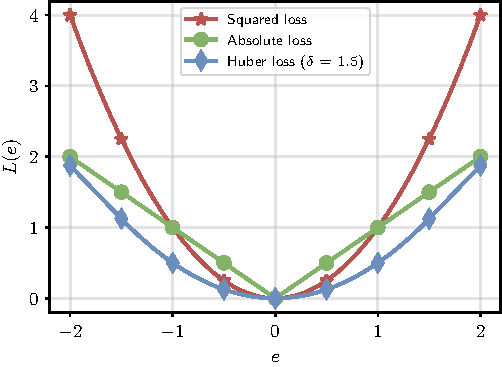
\includegraphics[width=0.6\textwidth]{images/loss_functions_regression.pdf}
    \caption{Визуализация квадратичной потери, потери по абсолютному значению и потери Хьюбера в зависимости от ошибки предсказания $e = (\hat{y} - y)$.}
    \label{fig:losses_regression}
\end{SCfigure}

которая является квадратичной вблизи ошибки $0$ и линейной в противном случае (с добавлением члена $-\frac{1}{2}$ для обеспечения непрерывности). См. Рисунок \ref{fig:losses_regression} для визуализации этих потерь в зависимости от ошибки предсказания. 

Потеря по абсолютному значению кажется неверным выбором в нашем контексте, поскольку у нее есть точка недифференцируемости в $0$ из-за абсолютного значения. Позже мы увидим, что функции с одной (или небольшим числом) точек такого вида не являются действительно проблематичными. Математически их можно обрабатывать с помощью понятия \textbf{субградиента} (небольшого обобщения производной). Практически вы можете представить, что если мы начнем со случайной инициализации, градиентный спуск никогда не достигнет этих точек с идеальной точностью, и производные $\lvert \varepsilon \rvert$ для любого $\varepsilon > 0$ всегда определены.

\subsection{Модель наименьших квадратов}
\label{subsec:least_squares}

\addclock Имея функцию потерь, мы рассмотрим следующую модель (линейную модель), чтобы завершить спецификацию нашей первой задачи обучения с учителем.
%
\begin{definition}[Линейные модели] 
A \textbf{линейная модель} на входе $\mathbf{x}$ определяется как:
%
$$
f(\mathbf{x})=\mathbf{w}^\top\mathbf{x} + b
$$
%
где $\mathbf{w} \sim (c)$ и $b \in \mathbb{R}$ (\textit{смещение}) являются обучаемыми параметрами.
\end{definition}

Интуиция заключается в том, что модель присваивает фиксированный вес $w_i$ каждому входному признаку $x_i$ и дает предсказание, линейно суммируя все эффекты для данного входа $\mathbf{x}$, возвращаясь к предсказанию по умолчанию, равному $b$, когда $\mathbf{x} = \mathbf{0}$. Геометрически модель определяет прямую для $d=1$, плоскость для $d=2$ и общую гиперплоскость для $d > 1$. С точки зрения нотации, мы иногда можем избежать написания члена смещения, предполагая постоянный член $1$ в качестве последнего признака $\mathbf{x}$:
%
$$
f\left(\begin{bmatrix}\mathbf{x}\\1\end{bmatrix}\right) = \mathbf{w}^\top\begin{bmatrix}\mathbf{x}\\1\end{bmatrix} = \mathbf{w}_{1:c}^\top\mathbf{x}+w_{c+1}
$$

Объединяя линейную модель, квадратичную потерю и задачу минимизации эмпирического риска, мы получаем \textbf{задачу оптимизации методом наименьших квадратов}.

\begin{definition}[Наименьшие квадраты] \addbottle
Задача оптимизации \textbf{методом наименьших квадратов} задается как:
%
\begin{equation}
\mathbf{w}^*, b^* = \underset{\mathbf{w}, b}{\arg\min} \;\;\frac{1}{n}\sum_{i=1}^n \left(y_i - \mathbf{w}^\top \mathbf{x}_i - b\right)^2
\label{eq:least_squares}
\end{equation}
\end{definition}

Прежде чем перейти к анализу этой задачи, мы перепишем наименьшие квадраты в \textbf{векторизованной} форме, которая включает только матричные операции (произведения матриц и нормы). Это полезно, потому что, как уже было сказано, современный код для обучения дифференцируемых моделей построен на основе $n$-мерных массивов с оптимизированным оборудованием для выполнения матричных операций над ними. Для этого мы сначала объединяем все входы и выходы нашего обучающего набора в \textbf{входную матрицу}:

$$
\mathbf{X} = \begin{bmatrix} \mathbf{x}_1^\top \\ \vdots \\ \mathbf{x}_n^\top \end{bmatrix} \sim (n,c)
$$

и аналогичный \textbf{выходной вектор} $y = \left[ y_1, \ldots, y_n\right]^\top$. Мы можем записать пакетный выход модели (выход модели для мини-пакета значений) как:

\begin{equation}
f(\mathbf{X})=\mathbf{X}\mathbf{w} + \eqnmarkbox[drawblue]{node}{\mathbf{1}b}
\label{eq:batched_linear_model}
\end{equation}
\annotate[yshift=-1em]{below,right}{node}{То же смещение $b$ для всех $n$ предсказаний}

\vspace{1em}
Уравнения, подобные \eqref{eq:batched_linear_model}, можно воспроизвести почти дословно в коде - см. Листинг \ref{code:linear_model} для примера в PyTorch. 

\begin{mypy}{Вычисление пакетной линейной модели, как в \protect\eqref{eq:batched_linear_model}. Для ясности мы показываем размеры массивов в виде подсказок типов с использованием {\footnotesize \texttt{jaxtyping} (\url{https://docs.kidger.site/jaxtyping/})}.}{code:linear_model}
def linear_model(w: Float[Tensor, "c"],
                 b: Float,
                 X: Float[Tensor, "n c"]) 
                 -> Float[Tensor, "n"]:
  return X @ w + b
\end{mypy}

Пока что это представляет лишь незначительный интерес, но будет более важным позже: мы отмечаем, что порядок строк входной матрицы и выходного вектора в основном произволен, в том смысле, что перестановка их строк приведет только к соответствующей перестановке строк $f(\mathbf{X})$. Это простой пример явления, называемого \textbf{перестановочной эквивариантностью}, которое будет играть гораздо более важную роль позже.

Векторизованная задача оптимизации методом наименьших квадратов становится:
%
\begin{equation}
\text{LS}(\mathbf{w},b) =  \frac{1}{n} \left\lVert \mathbf{y} - \mathbf{X}\mathbf{w} - \mathbf{1}b \right\rVert^2 
\label{eq:ls_vectorized}
\end{equation}
%
где мы напоминаем, что норма вектора определяется как $\lVert \mathbf{e} \rVert^2 = \sum_i e_i^2$.

\subsection{Решение задачи наименьших квадратов}

Чтобы решить задачу наименьших квадратов с помощью градиентного спуска, нам нужны уравнения для ее градиента. Хотя мы скоро разработаем общую алгоритмическую основу для автоматического вычисления этих градиентов (Глава \ref{chap:automatic_differentiation}), поучительно рассмотреть сам градиент в этом простом сценарии. Игнорируя смещение (по причинам, указанным выше, мы можем включить его в вектор весов) и другие постоянные члены, мы имеем:
%
$$
\nabla \text{LS}(\mathbf{w}) = \mathbf{X}^\top\left( \mathbf{X}\mathbf{w} - \mathbf{y} \right)
$$
%
Задача НК выпукла по весам модели, что можно неформально понять, заметив, что уравнения описывают параболоид в пространстве весов (квадратичную функцию). Глобальные минимумы тогда описываются уравнениями:
%
$$
\mathbf{X}^\top\left( \mathbf{X}\mathbf{w} - \mathbf{y} \right) = 0 \;\;\Rightarrow\;\; \mathbf{X}^\top\mathbf{X}\mathbf{w} = \mathbf{X}^\top\mathbf{y}
$$

\begin{mypy}{Решение задачи наименьших квадратов с помощью решения в замкнутой форме. Численно устойчивый вариант вызывает решатель, специализированный для систем линейных уравнений.}{code:ls_closed_form}
def least_squares_solve(w: Float[Tensor, "c"],
                        X: Float[Tensor, "n c"],
                        y: Float[Tensor, "n"],
                        numerically_stable = True) \
                        -> Float[Tensor, "c"]:
  # Явное решение
  if not numerically_stable:
    return torch.linalg.inv(X.T @ X) @ X.T @ y 
  else:
    return torch.linalg.solve(X.T @ X, X.T @ y)
\end{mypy}

Это называется \textbf{нормальными уравнениями}. Важно, что нормальные уравнения описывают линейную систему уравнений относительно $\mathbf{w}$,\footnote{То есть мы можем записать их как $\mathbf{A}\mathbf{w}=\mathbf{b}$, где $\mathbf{A} = \mathbf{X}^\top\mathbf{X}$ и $\mathbf{b} = \mathbf{X}^\top\mathbf{y}$.} что означает, что при соответствующих условиях (обратимости $\mathbf{X}^\top\mathbf{X}$) мы можем найти оптимальное решение как:
%
\begin{equation}
\mathbf{w}_*=\left(\mathbf{X}^\top\mathbf{X}\right)^{-1}\mathbf{X}^\top\mathbf{y}
\label{eq:ls_closed_form_solution}
\end{equation}

\begin{supportbox}{Интересные факты}
Матрица $\mathbf{X}^\dagger=\left(\mathbf{X}^\top\mathbf{X}\right)^{-1}\mathbf{X}^\top$ называется \textbf{псевдообратной} (или \textbf{обратной матрицей Мура-Пенроуза}) неквадратной матрицы $\mathbf{X}$, поскольку $\mathbf{X}^\dagger\mathbf{X}=\mathbf{I}$. Выполнение обращения в \eqref{eq:ls_closed_form_solution} не всегда возможно: например, если один признак является скалярным кратным другого, матрица $\mathbf{X}$ не имеет полного ранга (это называется \textbf{коллинеарностью}). Наконец, обратите внимание, что предсказания модели наименьших квадратов можно записать как $\hat{\mathbf{y}}=\mathbf{M}\mathbf{y}$, где $\mathbf{M} = \mathbf{X}\mathbf{X}^\dagger$. Следовательно, наименьшие квадраты также можно интерпретировать как выполнение взвешенного среднего обучающих меток, где веса задаются проекцией на пространство столбцов, индуцированное $\mathbf{X}$. Это называется \textbf{двойственной} формулировкой наименьших квадратов. Двойственные формулировки обеспечивают внутренний уровень отладки модели, поскольку они позволяют проверить, какие входы были наиболее релевантными для предсказания, проверив соответствующие двойственные веса \cite{irie2022dual}. 
\end{supportbox}

Это единственный случай, когда мы сможем выразить оптимальное решение в замкнутой форме, и поучительно сравнить это решение с решением, полученным градиентным спуском. Для этого мы показываем в Листинге \ref{code:ls_closed_form} пример решения задачи наименьших квадратов в замкнутой форме с использованием \eqref{eq:ls_closed_form_solution}, а в Листинге \ref{code:ls_gradient_descent} — эквивалентную формулировку с градиентным спуском. Прототипическая эволюция потерь в последнем случае показана на Рисунке \ref{fig:loss_evolution}. Поскольку мы выбрали очень малую скорость обучения, каждый шаг в процедуре градиентного спуска обеспечивает стабильное уменьшение потерь до сходимости. Практически сходимость можно проверить численными методами, например, оценив разницу в норме между двумя итерациями для некоторого числового порога $\varepsilon > 0$:
%
\begin{equation}
    \lVert \mathbf{w}_{t+1} - \mathbf{w}_t \rVert^2 < \varepsilon
\end{equation}
%
Как мы увидим, понимание того, когда более сложные модели сошлись, будет более тонкой задачей.

Рассматривая снова логарифм правдоподобия Гаусса в \eqref{eq:ls_maximum_likelihood}, мы также можем оптимизировать член по отношению к $\sigma^2$ после того, как веса были обучены, получая:
%
\begin{equation}
\sigma_*^{2} = \frac{1}{n}\sum_{i=1}^n (y_i - \mathbf{w}_*^{\top}\mathbf{x}_i)^2 \,.
\label{eq:ls_sigma}
\end{equation}
%
что имеет интуитивный смысл, что дисперсия модели постоянна (по определению) и задается средней квадратичной ошибкой предсказания на наших обучающих данных. Более сложные вероятностные модели можно получить, предположив, что сама дисперсия предсказывается моделью (\textbf{гетероскедастические} модели), см. \cite{bishop2006pattern}.

\begin{mypy}{Та же задача, что и в Листинге \protect\ref{code:ls_closed_form}, решенная с помощью наивной реализации градиентного спуска с фиксированной скоростью обучения, которая по умолчанию равна $\eta = 0.001$.}{code:ls_gradient_descent}
def least_squares_gd(X: Float[Tensor, "n c"],
                     y: Float[Tensor, "n"],
                     learning_rate=1e-3) \
                     -> Float[Tensor, "c"]:
    # Инициализация параметров
    w = torch.randn((X.shape[1], 1))

    # Фиксированное количество итераций
    for i in range(15000):
      # Обратите внимание на знак: производная имеет минус!
      w = w + learning_rate * X.T @ (y - X @ w)

    return w
\end{mypy}

\begin{SCfigure}
    \centering
    \hspace{1em} 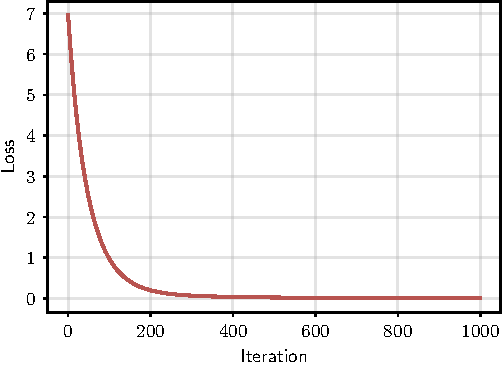
\includegraphics[width=0.5\textwidth]{images/least_squares_example.pdf}
    \caption{Пример выполнения кода из Листинга \ref{code:ls_closed_form}, где данные состоят из $n=10$ точек, взятых из линейной модели $\mathbf{w}^\top \mathbf{x} + \varepsilon$, с $w_i \sim \mathcal{N}(0, 1)$ и $\varepsilon \sim \mathcal{N}(0, 0.01)$. Детали в стороне, обратите внимание на очень плавный спуск: каждый шаг обеспечивает уменьшение потерь.}
    \label{fig:loss_evolution}
\end{SCfigure}


\subsection{Некоторые вычислительные соображения}

\addteacup Даже если обратную матрицу можно вычислить, качество решения будет зависеть от числа обусловленности $\mathbf{X}^\top\mathbf{X}$, и при плохо обусловленных матрицах могут возникать большие численные ошибки.\footnote{Число обусловленности матрицы $\mathbf{A}$ определяется как $\kappa(\mathbf{A}) = \lVert\mathbf{A}\rVert\lVert\mathbf{A}^{-1}\rVert$ для некоторого выбора матричной нормы $\lVert \bullet \rVert$. Большие числа обусловленности могут затруднить обращение, особенно если точность с плавающей запятой невысока.} Кроме того, вычислительная стоимость решения \eqref{eq:ls_closed_form_solution} может быть непомерно высокой. Обращение матрицы будет масштабироваться примерно как $\mathcal{O}(c^3)$. Что касается умножения матриц, алгоритм требует умножения матрицы $c \times n$ на другую матрицу $n \times c$ и умножения матрицы $c \times c$ на матрицу $c \times n$. Обе эти операции будут масштабироваться как $\mathcal{O}(c^2n)$.

В общем, мы всегда будем предпочитать алгоритмы, которые масштабируются линейно как по размерности признаков $c$, так и по размеру пакета $n$, поскольку сверхлинейные алгоритмы быстро станут непрактичными (например, пакет из $32$ RGB-изображений размером $1024 \times 1024$ имеет $c \approx 1e^{7}$). Мы можем избежать квадратичной сложности в уравнении градиента, вычисляя умножения в правильном порядке, т.е. сначала вычисляя произведение матрицы на вектор $\mathbf{X}\mathbf{w}$. Следовательно, чистый градиентный спуск линеен как по $c$, так и по $n$, но только при должном внимании к реализации: обобщение этой идеи является фундаментальным пониманием для разработки \textbf{автоматического дифференцирования в обратном режиме}, также известного как \textbf{обратное распространение ошибки} (Раздел \ref{sec:reverse_mode_automatic_differentiation}).

\subsection{Регуляризация решения методом наименьших квадратов}
\label{subsec:regularizing_least_squares}

Снова взглянув на потенциальную нестабильность операции обращения, предположим, у нас есть набор данных, для которого матрица почти сингулярна, но мы все же хотим продолжить с решением в замкнутой форме. В этом случае можно немного изменить задачу, чтобы получить решение, которое «как можно ближе» к исходному, но при этом его можно вычислить. Например, известный трюк — добавить небольшое кратное, $\lambda > 0$, единичной матрицы к обращаемой матрице:
%
$$
\mathbf{w}^*=\left(\mathbf{X}^\top\mathbf{X} {\color{drawred}+\lambda\mathbf{I}}\right)^{-1}\mathbf{X}^\top\mathbf{y}
$$
%
Это подталкивает матрицу к тому, чтобы она была «более диагональной», и улучшает ее число обусловленности. Возвращаясь к исходной задаче, мы отмечаем, что это решение в замкнутой форме для измененной задачи оптимизации:
%
$$
\text{LS-Reg}(\mathbf{w}) =  \frac{2}{n} \left\lVert \mathbf{y} - \mathbf{X}\mathbf{w} \right\rVert^2 {\color{drawred}+ \frac{\lambda}{2}\lVert \mathbf{w} \rVert^2}
$$
%
Эта задача называется \textbf{регуляризованными наименьшими квадратами} (или \textbf{гребневой регрессией}), и красная часть в потерях является примером $\ell_2$-регуляризации (или, в более общем смысле, регуляризации). Обратите внимание, что регуляризация не зависит от набора данных, поскольку она просто кодирует предпочтение определенного типа решения (в данном случае, весов с малой нормой), где сила самого предпочтения определяется гиперпараметром $\lambda$. С байесовской точки зрения (Раздел \ref{sec:bayesian_learning}), регуляризованные наименьшие квадраты соответствуют решению MAP при определении гауссовского априорного распределения над весами с центром в нуле и постоянной дисперсией.

\section{Линейные модели для классификации}
\label{sec:linear_models_for_classification}

Теперь мы переходим к классификации, в которой $y_i \in \left\{1, \ldots, m\right\}$, где $m$ определяет количество \textbf{классов}. Как мы увидим позже, это очень влиятельная задача, охватывающая широкий круг задач как в компьютерном зрении (например, классификация изображений), так и в обработке естественного языка (например, предсказание следующего токена). Мы можем решить эту задачу с помощью небольших вариаций по сравнению с регрессионным случаем.

Хотя мы можем решить задачу, регрессируя непосредственно на целочисленное значение $y_i$, поучительно рассмотреть, почему это может быть не лучшей идеей. Во-первых, модели трудно напрямую предсказывать целочисленное значение, поскольку это требует некоторого порогового значения, которое сделало бы ее градиент почти везде равным нулю. Вместо этого мы могли бы регрессировать на вещественное значение $\widetilde{y}_i \in \left[1, m\right]$ внутри интервала от $1$ до $m$ (как мы покажем, ограничение выхода модели внутри интервала можно легко сделать). Во время вывода, для выхода $\hat{y}_i = f(\mathbf{x}_i)$, мы отображаем обратно в исходную область путем округления:
%
$$
\text{Предсказанный класс} =\text{round}(\hat{y}_i)
$$
%
Например, $\hat{y}_i = 1.3$ будет отображено в класс $1$, а $\hat{y}_i = 3.7$ — в класс $4$. Обратите внимание, что это постобработка значений, которая возможна только во время вывода. Причина, по которой это не лучший выбор моделирования, заключается в том, что мы вводим ложный порядок классов, который может быть использован самой моделью, где класс $2$ «ближе» к классу $3$ чем к классу $4$. Мы можем избежать этого, перейдя к классической \textbf{one-hot закодированной} версии $y$, которую мы обозначаем как $\mathbf{y}^{\text{oh}} \sim \text{Binary}(m)$:
%
$$
\idx{\mathbf{y}^{\text{oh}}}{j}=\begin{cases} 1 &\text{ если } y = j \\ 0 & \text{ иначе} \end{cases}
$$
%
Например, в случае трех классов мы имели бы $\mathbf{y}^{\text{oh}} = \left[1 \;\; 0 \;\; 0 \right]^\top$ для класса $1$, $\mathbf{y}^{\text{oh}} = \left[0 \;\; 1 \;\; 0 \right]^\top$ для класса $2$ и $\mathbf{y}^{\text{oh}} = \left[0 \;\; 0 \;\; 1 \right]^\top$ для класса $3$ (это представление должно быть знакомо читателям с некоторым опытом в машинном обучении, поскольку это стандартное представление для категориальных переменных). 

One-hot векторы неупорядочены, в том смысле, что для двух общих выходов $\mathbf{y}_1^{\text{oh}}$ и $\mathbf{y}_2^{\text{oh}}$ их евклидово расстояние равно либо $0$ (тот же класс), либо $\sqrt{2}$ (разные классы). Хотя мы можем выполнять многозначную регрессию непосредственно на one-hot закодированных выходах, со среднеквадратичной ошибкой, известной в этом случае как \textbf{оценка Брайера}, мы покажем ниже, что существует лучшее и более элегантное решение в виде \textbf{логистической регрессии}.

\subsection{Симплекс вероятностей и функция softmax}
\label{sec:softmax}

Мы не можем обучить модель напрямую предсказывать one-hot закодированный вектор (по тем же причинам, что и выше), но мы можем достичь чего-то подобного с помощью небольшого ослабления. Для этого мы снова вводим \textbf{симплекс вероятностей}.

\begin{definition}[Симплекс вероятностей]
\textbf{Симплекс вероятностей} $\Delta_n$ — это множество векторов $\mathbf{x} \sim \Delta(n)$ таких, что:
%
$$
x_i \ge 0, \; \sum_i x_i=1
$$
%
\end{definition}

Геометрически вы можете представить множество one-hot векторов как вершины $n$-мерного многогранника, а симплекс — как его выпуклую оболочку: значения внутри симплекса, такие как $[0.2, 0.05, 0.75]$, не соответствуют точно вершине, но они позволяют использовать градиентный спуск, потому что мы можем плавно перемещаться внутри многогранника. Для значения $\mathbf{x} \in \Delta_n$ мы можем спроецировать на его ближайшую вершину (предсказанный класс) как:
%
$$
\underset{i}{\arg\max} \left\{ \mathbf{x}_i \right\}
$$
%
Как следует из названия, мы можем интерпретировать значения внутри симплекса как распределения вероятностей, а проекцию на ближайшую вершину — как нахождение моды (наиболее вероятного класса) в распределении. В этой интерпретации one-hot закодированный вектор является «особым случаем», когда вся масса вероятности сосредоточена на одном классе (который, как мы знаем, является правильным).

Чтобы предсказать значение в этом симплексе, нам нужны две модификации линейной модели из \eqref{eq:least_squares}: во-первых, нам нужно предсказать целый вектор одновременно; и во-вторых, нам нужно ограничить выходы, чтобы они лежали в симплексе. Во-первых, мы модифицируем линейную модель для предсказания $m$-мерного вектора:
%
\begin{equation}
\mathbf{y} =\mathbf{W}\mathbf{x}+\mathbf{b}
\label{eq:multi_valued_linear_model}
\end{equation}
%
где $\mathbf{W} \sim (m,c)$ можно интерпретировать как $m$ линейных регрессионных моделей, работающих параллельно, и $\mathbf{b} \sim(m)$. Этот выход неограничен и не гарантированно находится в симплексе. Идея логистической регрессии заключается в том, чтобы объединить линейную модель в \eqref{eq:multi_valued_linear_model} с простой, безпараметрической трансформацией, которая проецирует внутрь симплекса, называемой функцией \textbf{softmax}.

\begin{definition}[Функция Softmax] \addbottle
Функция \textbf{softmax} определяется для общего вектора $\mathbf{x} \sim(m)$ как:

\begin{equation}
\idx{\textnormal{softmax}(\mathbf{x})}{i} = \frac{\exp(x_i)}{\sum_j\exp(x_j)}
\label{eq:softmax}
\end{equation}

\end{definition}

Давайте разложим члены в \eqref{eq:softmax} на основные вычисления, которые выполняются, введя два промежуточных члена. Во-первых, числитель softmax преобразует каждое число в положительное значение $h_i$ путем возведения в степень:
%
\begin{equation}
h_i =\exp(x_i)
\end{equation}
%
Во-вторых, мы вычисляем нормировочный коэффициент $Z$ как сумму этих новых (неотрицательных) значений:
%
\begin{equation}
 Z = \sum_jh_j 
 \end{equation}
%
Выход softmax затем задается делением $h_i$ на $Z$, тем самым гарантируя, что новые значения суммируются в $1$:
%
\begin{equation}
y_i = \frac{h_i}{Z}
\end{equation}

Другая перспектива открывается при рассмотрении более общей версии softmax, где мы добавляем дополнительный гиперпараметр $\tau > 0$, называемый \textbf{температурой}:

$$
\text{softmax}(\mathbf{x};\tau)=\text{softmax}(\mathbf{x}/\tau)
$$

Softmax сохраняет относительный порядок между значениями $x_i$ для всех значений $\tau$, но их абсолютное расстояние увеличивается или уменьшается в зависимости от температуры. В частности, у нас есть следующие два предельных случая:

\begin{gather}
\lim_{\tau \rightarrow \infty} \text{softmax}(\mathbf{x};\tau)=1/c \\
\lim_{\tau \rightarrow 0} \text{softmax}(\mathbf{x};\tau)=\underset{i}{\arg\max} \;\; \mathbf{x}
\end{gather}

При бесконечной температуре относительные расстояния исчезнут, и выход вернется к равномерному распределению. Напротив, при температуре $0$ softmax возвращается к (плохо дифференцируемой) операции argmax. Следовательно, softmax можно рассматривать как простое дифференцируемое приближение к argmax, и лучшим названием было бы \textbf{softargmax}. Однако мы будем придерживаться здесь наиболее стандартного названия. См. Рисунок \ref{fig:softmax} для визуализации softmax, примененного к общему трехмерному вектору с различными значениями температуры.

\begin{figure}[t]
    \centering
    \begin{subfigure}[b]{0.24\textwidth}
    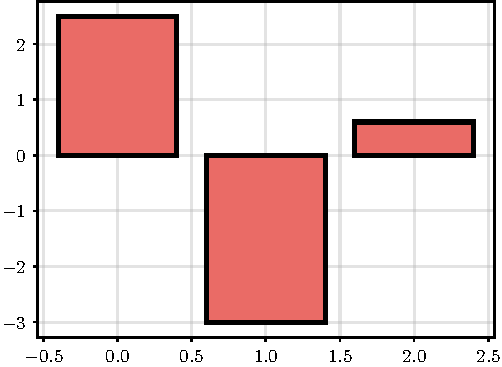
\includegraphics[width=\textwidth]{images/softmax_1.pdf}
    \caption{Входы}
    \end{subfigure}
    \hfill
    \begin{subfigure}[b]{0.24\textwidth}
    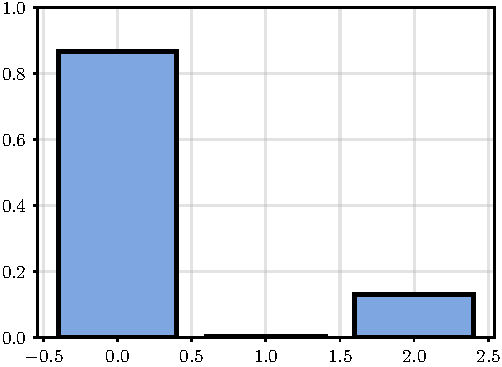
\includegraphics[width=1.0\textwidth]{images/softmax_2.pdf}
    \caption{$\tau=1$}
    \end{subfigure}
    \hfill
    \begin{subfigure}[b]{0.24\textwidth}
    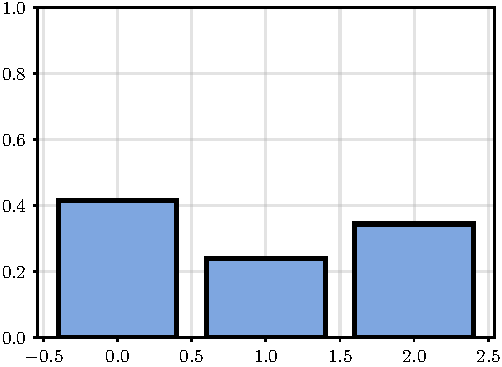
\includegraphics[width=1.0\textwidth]{images/softmax_3.pdf}
    \caption{$\tau=10$}
    \end{subfigure}
    \hfill
    \begin{subfigure}[b]{0.24\textwidth}
    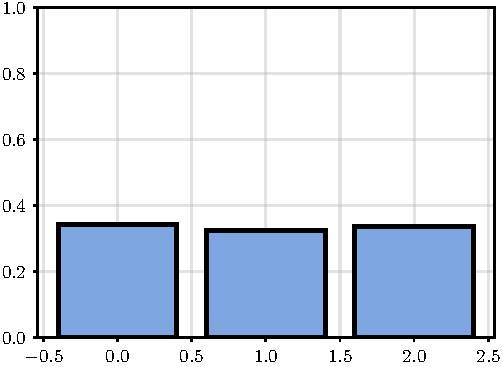
\includegraphics[width=1.0\textwidth]{images/softmax_4.pdf}
    \caption{$\tau=100$}
    \end{subfigure}
    \hfill
    \caption{Пример применения softmax к трехмерному вектору (a), с температурой, установленной в 1 (b), 10 (c) и 100 (d). По мере увеличения температуры выход сходится к равномерному распределению. Обратите внимание, что входы могут быть как положительными, так и отрицательными, но выходы softmax всегда ограничены в $[0,1]$.}
    \label{fig:softmax}
\end{figure}


\subsection{Модель логистической регрессии}
\label{subsec:logistic_regression}

\addclock Мы можем обобщить наше предыдущее обсуждение, объединив softmax в \eqref{eq:softmax} с линейной моделью в \eqref{eq:multi_valued_linear_model}, чтобы получить линейную модель для классификации:

$$
\hat{\mathbf{y}}=\text{softmax}\left(\mathbf{W}\mathbf{x} + \mathbf{b}\right)
$$

Предварительно нормализованные выходы $\mathbf{h} = \mathbf{W}\mathbf{x}+\mathbf{b}$ называются \textbf{логитами} модели, название, которое будет более подробно обсуждаться в следующем разделе. 

Единственное, что осталось для завершения спецификации модели логистической регрессии, — это функция потерь. Мы можем легко достичь этого, рассмотрев вероятностную точку зрения из Раздела \ref{subsec:how_to_select_a_loss}. Поскольку наши выходы ограничены симплексом вероятностей, мы можем интерпретировать их как параметры категориального распределения:

\vspace{1em}
\begin{equation*}
p(\eqnmarkbox[drawblue]{node}{\mathbf{y}^{\text{oh}}}\;\vert\;\hat{\mathbf{y}}) = \prod_i \hat{y}_i^{\eqnmarkbox[drawred]{node2}{y_i^{\text{oh}}}}
\end{equation*}
\annotate[yshift=1em]{above,left}{node2}{Степень всегда либо $0$, либо $1$}
\annotate[yshift=-1em]{below,right}{node}{One-hot закодированный класс}

Вычисление решения по максимальному правдоподобию в этом случае (попробуйте) дает нам \textbf{кросс-энтропийную потерю}.

\begin{definition}[Кросс-энтропийная потеря] \addbottle
Функция потерь \textbf{кросс-энтропии} между $\mathbf{y}^{\text{oh}}$ и $\hat{\mathbf{y}}$ задается как:
%
\begin{equation}
\textnormal{CE}(\mathbf{y}^{\textnormal{oh}},\hat{\mathbf{y}})= - \sum_i y_i^{\textnormal{oh}}\log(\hat{y}_i)
\label{eq:cross_entropy}
\end{equation}
\end{definition}

Потери также можно вывести как дивергенцию Кульбака-Лейблера между двумя распределениями вероятностей. Хотя на первый взгляд это неинтуитивно, у этого есть очень простое толкование, если заметить, что только одно значение $\mathbf{y}^{\text{oh}}$ будет ненулевым, соответствующее истинному классу $y = \underset{i}{\arg\max} \left\{ y^{\text{oh}}_i \right\}$. Тогда мы можем упростить потери как:

\begin{equation}
\text{CE}(y, \hat{\mathbf{y}}) = - \log(\eqnmarkbox[drawred]{node}{\hat{y}_y})
\label{eq:ce_single_term}
\end{equation}
\annotate[yshift=1em]{above,right}{node}{Вероятность, присвоенная истинному классу}


Из \eqref{eq:ce_single_term} мы видим, что эффект минимизации потерь CE заключается в максимизации выходной вероятности, соответствующей истинному классу. Это работает, поскольку из-за знаменателя в softmax любое увеличение одного выходного члена автоматически приведет к уменьшению других членов. Собирая все вместе, мы получаем задачу оптимизации логистической регрессии:
%
$$
\text{LR}(\mathbf{W},\mathbf{b})=\frac{1}{n}\sum_{i=1}^n \text{CE}\left( \mathbf{y}_i^{\text{oh}}, \text{softmax}(\mathbf{W}\mathbf{x}_i+\mathbf{b}) \right) \,.
$$
%
В отличие от наименьших квадратов, мы больше не можем вычислить решение в замкнутой форме, но мы все еще можем использовать градиентный спуск. В следующем разделе мы покажем пример градиента в этом случае, а в Разделе \ref{sec:reverse_mode_automatic_differentiation} — общую технику вычисления градиентов в таких случаях.

\section{Дополнительные темы по классификации}

\subsection{Бинарная классификация}

Рассмотрим теперь конкретный случай $m=2$. В этом случае у нас $y \in \left\{0,1\right\}$, и задача сводится к \textbf{бинарной классификации}, иногда называемой \textbf{обучением понятий} (поскольку нам нужно научиться, присутствует или отсутствует в входе определенное бинарное «понятие»). При стандартной логистической регрессии это моделировалось бы функцией с двумя выходами. Однако из-за знаменателя softmax последний выход логистической регрессии всегда избыточен, поскольку его можно вывести, зная, что выходы должны суммироваться в $1$:
%
$$
f_m(\mathbf{x}) = \sum_{i=1}^{m-1}f_i(\mathbf{x})
$$
%
Исходя из этого, мы можем немного упростить формулировку, рассмотрев скалярную модель с одним выходом $f(\mathbf{x}) \in [0,1]$, так что:
%
$$
\text{Предсказанный класс} = \text{round}(f(\mathbf{x}))= \begin{cases} 0 & \text{ если } f(\mathbf{x}) \le 0.5 \\ 1 & \text{ иначе } \end{cases} 
$$
%
Чтобы достичь желаемой нормализации в $[0,1]$, первый выход двузначного softmax можно переписать как $\frac{\exp(x_1)}{1+\exp(x_1)}$, и мы можем еще упростить его, разделив обе стороны на $\exp(x_1)$. Результатом является функция \textbf{сигмоида}.

\begin{definition}[Функция сигмоида] \addbottle
Функция \textbf{сигмоида} $\sigma(s) : \mathbb{R} \rightarrow [0,1]$ задается как:
%
$$
\sigma(s)=\frac{1}{1+\exp(-s)}
$$
%
\end{definition}

Сигмоида обеспечивает общее преобразование, проецирующее любое вещественное значение в интервал $[0,1]$ (с двумя крайними значениями, достигаемыми только асимптотически). Ее график показан на Рисунке \ref{fig:sigmoid}.

\begin{SCfigure}
    \centering
    \hspace{1em}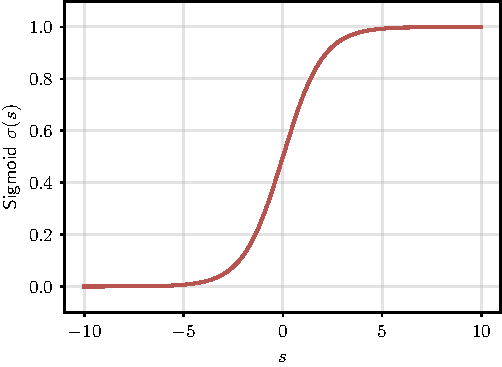
\includegraphics[width=0.6\textwidth]{images/sigmoid.pdf}
    \caption{График функции сигмоида. Обратите внимание, что $\sigma(0)=0.5$.}
    \label{fig:sigmoid}
\end{SCfigure}

Модель \textbf{бинарной логистической регрессии} получается путем объединения одномерной линейной модели с сигмоидальным масштабированием выхода:
%
$$
f(\mathbf{x})=\sigma\left(\mathbf{w}^\top\mathbf{x}+b\right)
$$
%
Кросс-энтропия аналогично упрощается до:

\vspace{1em}
\begin{equation}
\text{CE}(\hat{y},y) = \eqnmarkbox[drawred]{node}{-y\log(\hat{y})} \eqnmarkbox[drawblue]{node2}{-(1-y)\log(1-\hat{y})}
\end{equation}
\annotate[yshift=1em]{above,left}{node}{Потери для класса $1$}
\annotate[yshift=1em]{above,right}{node2}{Потери для класса $2$}

Следовательно, в случае бинарной классификации мы можем решить задачу двумя эквивалентными подходами: (а) двузначной моделью со стандартным softmax или (б) упрощенным однозначным выходом с сигмоидальным преобразованием выхода. 

В качестве интересного примечания рассмотрим градиент модели бинарной логистической регрессии по отношению к $\mathbf{w}$ (аналогичный градиент можно также записать для стандартного многоклассового случая):
%
$$
\nabla \text{CE}(f(\mathbf{x}),y) = (f(\mathbf{x})-y)\mathbf{x}
$$
%
Обратите внимание на сходство с градиентом стандартной линейной модели для регрессии. Это сходство можно лучше понять, переписав нашу модель как:

\vspace{1em}
\begin{equation}
\eqnmarkbox[drawred]{node}{\mathbf{w}^\top \mathbf{x}+b}=\eqnmarkbox[drawblue]{node2}{\log\left(\frac{y}{1-y}\right)}
\end{equation}
\annotate[yshift=1em]{above,left}{node}{Логиты}
\annotate[yshift=1em]{above,right}{node2}{Обратная сигмоида: $\sigma^{-1}(y)$}

Это проясняет, почему мы называли модель «линейной моделью» для классификации: мы всегда можем переписать ее как чисто линейную модель в терминах нелинейного преобразования выхода (в данном случае, обратной сигмоиды, также известной как \textbf{лог-отношение шансов}). Фактически, модель логистической регрессии является частью более широкого семейства моделей, расширяющих эту идею, называемых \textbf{обобщенными линейными моделями}. Для любознательного читателя название логита можно понять в этом контексте в связи с функцией пробита.\footnote{\url{https://en.wikipedia.org/wiki/Probit}}

\subsection{Трюк с logsumexp} 

\addteacup Это более технический подраздел, который проясняет аспект реализации того, что мы описали до сих пор. Глядя на фреймворки, такие как TensorFlow или PyTorch, мы можем найти несколько существующих реализаций кросс-энтропийной потери, основанных на том, описывается ли выход как целое число или как one-hot закодированный вектор. Это можно легко понять, поскольку мы уже видели, что можем сформулировать кросс-энтропийную потерю в обоих случаях. Однако мы также можем найти варианты, которые принимают логиты вместо нормализованных softmax выходов, как показано в Листинге \ref{code:cross_entropy}.

\begin{mypy}{Потери кросс-энтропии в PyTorch. Некоторые потери определены только начиная с логитов модели, а не с выхода после softmax. Это \textit{функциональные} варианты потерь - эквивалентные объектно-ориентированные варианты также присутствуют в большинстве фреймворков.}{code:cross_entropy}
# Бинарная кросс-энтропия
torch.nn.functional.binary_cross_entropy
# Бинарная кросс-энтропия, принимающая логиты
torch.nn.functional.binary_cross_entropy_with_logits
# Стандартная кросс-энтропия, работает только с логитами
torch.nn.functional.cross_entropy
# Кросс-энтропия, принимающая log f(x) в качестве входов
torch.nn.functional.nll_loss
\end{mypy}

Чтобы понять, зачем нам это нужно, рассмотрим $i$-й член кросс-энтропии в терминах логитов $\mathbf{p}$:
%
$$
- \log\left( \frac{\exp{p_i}}{\sum_j \exp{p_j}} \right) \,.
$$
%
Этот член может вызывать несколько численных проблем, в частности из-за взаимодействия между (потенциально неограниченными) логитами и возведением в степень. Чтобы решить это, мы сначала перепишем его как:
%
$$
- \log\left( \frac{\exp{p_i}}{\sum_j \exp{p_j}} \right) = -p_i + \underbrace{\log\left(\sum_j \exp p_j\right)}_{\triangleq \; \text{logsumexp}(\mathbf{p})}
$$
%
Первый член не страдает от нестабильности, в то время как второй член (\textbf{logsumexp} логитов) является функцией всего вектора логитов, и можно показать, что он инвариантен для данного скаляра $c \ge 0$ в следующем смысле:\footnote{\url{https://gregorygundersen.com/blog/2020/02/09/log-sum-exp/}}
%
$$
\text{logsumexp}(\mathbf{p})=\text{logsumexp}(\mathbf{p} - c) +c
$$
%
Обратите внимание, что $\nabla \text{softmax}(\bullet) = \text{logsumexp}(\bullet)$. Взяв $c = \max(\mathbf{p})$, мы можем предотвратить численные проблемы, ограничив максимальное значение логита $0$. Однако это возможно только в том случае, если у нас есть доступ к исходным логитам, поэтому численно стабильные варианты кросс-энтропии требуют их в качестве входных данных. Это создает небольшую двусмысленность, поскольку softmax теперь может быть включен либо как часть модели, либо как часть функции потерь.

\subsection{Калибровка и классификация}

Мы завершаем главу кратким обсуждением важной темы \textbf{калибровки} классификатора. Чтобы понять это, рассмотрим следующий факт: хотя наша модель предоставляет целое распределение по возможным классам, наш критерий обучения нацелен только на максимизацию истинного класса. Следовательно, следующее предложение оправдано:

\begin{quote}Предсказанный класс $f(\mathbf{x})$ — это $\underset{i}{\arg\max} \; \idx{f(\mathbf{x})}{i}$.\end{quote}

Вместо этого это более общее предложение может быть неверным:

\begin{quote} Вероятность того, что $\mathbf{x}$ относится к классу $i$, равна $\idx{f(\mathbf{x})}{i}$.\end{quote}

Когда оценки уверенности сети совпадают с вероятностью того, что данное предсказание верно, мы говорим, что выходы сети \textbf{откалиброваны}.

\begin{definition}[Калибровка]
Классификационная модель $f(\mathbf{x})$, выдающая на выходе вероятности классов, называется откалиброванной, если для любого возможного предсказания выполняется следующее:
%
$$
\idx{f(\mathbf{x})}{i} = p(y=i \;\vert\; \mathbf{x})
$$
%
\end{definition}

Хотя кросс-энтропия должна восстанавливать условное распределение вероятностей для неограниченного класса моделей и в пределе бесконечных данных \cite{hastie2009elements}, на практике несоответствие между ними может быть высоким \cite{blasiok2024does}, особенно для более сложных моделей, которые мы представим позже.

Чтобы понять разницу между точностью и калибровкой, рассмотрим два сценария. Во-первых, рассмотрим модель бинарной классификации с идеальной точностью, но всегда предсказывающую истинный класс с уверенностью $0.8$. В этом случае модель явно \textit{недоуверена} в своих предсказаниях, поскольку, глядя на уверенность, мы можем предположить, что $20\%$ из них будут неверными. Во-вторых, рассмотрим задачу с 4 классами с идеально сбалансированными классами, с моделью, которая всегда предсказывает $[0.25, 0.25, 0.25, 0.25]$. В этом случае модель идеально откалибрована, но бесполезна с точки зрения точности.

Наличие откалиброванной модели очень важно в ситуациях, когда разные предсказания могут иметь разную стоимость. Это можно формализовать, определив так называемую \textit{матрицу стоимости}, присваивающую стоимость $C_{ij}$ для любого входа класса $i$, предсказанного как класс $j$. Стандартным примером является задача бинарной классификации с матрицей стоимостей, показанной в Таблице \ref{tab:cost_matrix}.

%
\begin{table}[h]
\centering
\caption{Пример матрицы стоимости для задачи классификации с асимметричными стоимостями ошибочной классификации.}
\label{tab:cost_matrix}
\begin{tabular}{@{}lcc@{}}
\toprule
 & Истинный класс 0 & Истинный класс 1 \\ \midrule
Предсказанный класс 0 & 0 & 10 \\
Предсказанный класс 1 & 1 & 0 \\ \bottomrule
\end{tabular}
\end{table}

Мы можем интерпретировать Таблицу \ref{tab:cost_matrix} следующим образом: правильное предсказание не несет затрат, в то время как ошибка ложноотрицательного предсказания (0 вместо 1) в 10 раз дороже, чем ошибка ложноположительного предсказания. Например, неверная ложноотрицательная ошибка в медицинском диагнозе намного хуже, чем ложноположительная ошибка, при которой дальнейшее обследование может исправить ошибку. Откалиброванная модель может помочь нам лучше оценить средний риск ее развертывания и настроить баланс между ложноположительными и ложноотрицательными ошибками.

Чтобы увидеть это, обозначим через $\mathbf{C} \sim (m, m)$ общую матрицу стоимостей для многоклассовой задачи (например, матрицу $2\times2$ в Таблице \ref{tab:cost_matrix}). Рациональным выбором является выбор класса, который минимизирует ожидаемую стоимость на основе оценок, присвоенных нашей моделью:
%
$$
\underset{i}{\arg\min} \sum_{j=1}^m C_{ij} \idx{f(\mathbf{x})}{j}
$$
%
Если $C_{ij} = 1$, когда $i \neq j$, и $0$ в противном случае, это сводится к выбору argmax $f$, но для общей матрицы стоимостей выбор предсказанного класса будет зависеть от относительных стоимостей совершения конкретных ошибок. Это простой пример \textbf{теории принятия решений} \cite{bishop2006pattern}.

\subsection{Оценка ошибки калибровки}

Чтобы оценить, откалибрована ли модель, мы можем разбить ее предсказания на интервалы и сравнить ее калибровку с точностью в каждом интервале. Для этого предположим, что мы разделили интервал $[0,1]$ на $b$ равноотстоящих интервалов, каждый размером $1/b$. Возьмем проверочный набор размером $n$ и обозначим через $\mathcal{B}_i$ элементы, чья уверенность попадает в интервал $i$. Для каждого интервала мы можем дополнительно вычислить среднюю уверенность $p_i$ модели (которая будет примерно в середине интервала) и среднюю точность $a_i$. Построение графика пар $(a_i, p_i)$ на гистограмме называется \textbf{диаграммой надежности}, как показано на Рисунке \ref{fig:calibration_plot}. Чтобы иметь единую скалярную метрику калибровки, мы можем использовать, например, \textbf{ожидаемую ошибку калибровки} (ECE):

\begin{SCfigure}
    \centering
    \hspace{1em}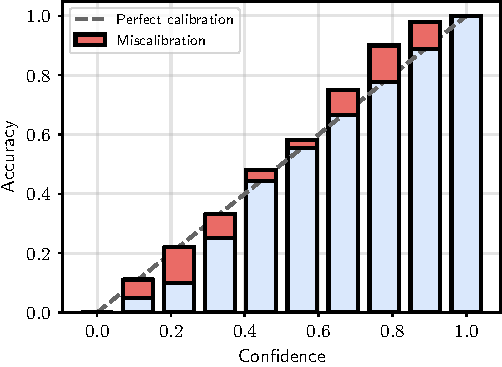
\includegraphics[width=0.5\textwidth]{images/reliability_plot.pdf}
    \caption{Пример диаграммы надежности с $b=10$ интервалами. Синие столбцы показывают среднюю точность модели в этом интервале, а красные столбцы показывают ошибку калибровки для интервала, которая может быть либо недооцененной (ниже диагонали), либо переоцененной (выше диагонали). Взвешенная сумма красных блоков — это ECE в \eqref{eq:ece}.}
    \label{fig:calibration_plot}
\end{SCfigure}

\begin{equation}
\displaystyle\text{ECE}= \sum_i \eqnmarkbox[drawred]{node2}{\frac{\lvert\mathcal{B}_i\rvert}{n}} \eqnmarkbox[drawblue]{node}{\left|a_i - p_i\right|}
\label{eq:ece}
\end{equation}
\annotate[yshift=1em]{above,right}{node}{Калибровка для интервала $i$}
\annotate[yshift=-1em]{below,right}{node2}{Доля проверочного набора, попадающая в интервал $i$}

\vspace{1em}
Возможны и другие метрики, такие как максимум по интервалам. Если модель оказывается неоткалиброванной, необходимо внести изменения. Примеры включают перемасштабирование предсказаний с помощью температурного масштабирования \cite{guo2017calibration} или оптимизацию с другой функцией потерь, такой как фокальная потеря \cite{mukhoti2020calibrating}.

В заключение мы упомянем альтернативу прямой калибровке модели, называемую \textbf{конформным предсказанием}, которая стала популярной в последнее время \cite{angelopoulos2021gentle}. Предположим, мы фиксируем порог $\gamma$ и берем множество классов, предсказанных моделью, чья соответствующая вероятность выше $\gamma$:
%
\begin{equation}
\mathcal{C}(\mathbf{x}) = \left\{ i \mid \idx{f(\mathbf{x})}{i} > \gamma \right\}
\label{eq:support_set}
\end{equation}

\begin{SCfigure}
    \centering
    \hspace{1em}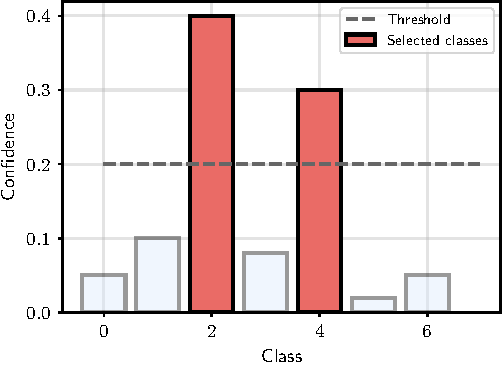
\includegraphics[width=0.5\textwidth]{images/conformal_prediction.pdf}
    \caption{Калибровка путем превращения выхода модели в множество: мы возвращаем все классы, чья предсказанная вероятность превышает заданный порог. Правильно выбрав порог, мы можем ограничить вероятность нахождения истинного класса в выходном множестве.}
    \label{fig:conformal_prediction}
\end{SCfigure}

т.е. ответ модели теперь является \textit{множеством} $\mathcal{C}(\mathbf{x})$ потенциальных классов. Пример показан на Рисунке \ref{fig:conformal_prediction}. Идея конформного предсказания заключается в выборе минимального $\gamma$ такого, что вероятность нахождения правильного класса $y$ в множестве выше определенной пользователем ошибки $\alpha$:\footnote{Обратите внимание, что всегда возможно удовлетворить это свойство, выбрав $\gamma = 0$, т.е. включив все классы в выходное множество:}
%
\begin{equation}
p(y \in \mathcal{C}(\mathbf{x})) \ge 1 -\alpha
\label{eq:conformal_prediction}
\end{equation}
%
Интуитивно, существует обратно пропорциональная зависимость между $\gamma$ и $\alpha$. Конформное предсказание предоставляет автоматические алгоритмы для гарантии \eqref{eq:conformal_prediction} за счет того, что на выходе больше нет одного класса.

\section*{От теории к практике}

\begin{wrapfigure}{r}{3.0cm}
\vspace{-3em}
\includegraphics[width=3.0cm]{images/shutterstock_2075221579.jpg}
\vspace{-6em}
\end{wrapfigure}

Из Главы \ref{chap:preliminaries} вы должны хорошо разбираться в NumPy, JAX и \mintinline{python}{torch.tensor} из PyTorch. Все они подходят для этой главы, и больше ничего не требуется.

Я предлагаю короткое упражнение, чтобы вы могли обучить свою первую дифференцируемую модель:

\begin{enumerate}
\item Загрузите игрушечный набор данных: например, один из тех, что содержатся в модуле наборов данных scikit-learn.\footnote{\url{https://scikit-elearn.org/stable/datasets/toy_dataset.html}}
\item Постройте линейную модель (для регрессии или классификации в зависимости от набора данных). Подумайте, как сделать код как можно более модульным: как мы увидим, вам понадобится как минимум две функции, одна для инициализации параметров модели и одна для вычисления предсказаний модели.
\end{enumerate}

\begin{enumerate}\addtocounter{enumi}{2}
\item Обучите модель с помощью градиентного спуска. Пока вы можете вычислять градиенты вручную: попробуйте представить, как вы можете сделать и эту часть модульной, т.е. как вы измените вычисление градиента, если захотите динамически добавлять или удалять смещение из модели?
\item Постройте график функции потерь и точности на независимом тестовом наборе. Если вы знакомы со стандартным машинным обучением, вы можете сравнить результаты с другими моделями обучения с учителем, такими как дерево решений или $k$-NN, всегда используя scikit-learn.
\end{enumerate}
